\documentclass{article}

% Language setting
% Replace `english' with e.g. `spanish' to change the document language
\usepackage[english]{babel}

% Set page size and margins
% Replace `letterpaper' with `a4paper' for UK/EU standard size
\usepackage[letterpaper,top=2cm,bottom=2cm,left=3cm,right=3cm,marginparwidth=1.75cm]{geometry}

% Useful packages
\usepackage{amsmath}
\usepackage{authblk}
\usepackage{lmodern}
\usepackage{graphicx}
\usepackage{todonotes}
\usepackage{placeins}   % helps to keeps figures at the same page or within the /FloatBarrier
\usepackage{caption}    % lets you define the fontsize of figure captions
\usepackage{subcaption}
\usepackage[colorlinks=true, allcolors=blue]{hyperref}

%added by LK
\usepackage{textgreek}
\usepackage{ltablex} %have centerised tables
%\usepackage{subfig}

\renewcommand\Authfont{\fontsize{9}{10}\selectfont}
\renewcommand\Affilfont{\fontsize{8}{9}\itshape}

\title{Implementation of an On-Board Terrain Classifier based on Proprioceptive Sensor Data for a Planetary Rover}
\author[1]{Raul Dominguez}
\author[2]{Lennart Kuhr}
\author[1]{Jonathan Babel}
\author[1]{Florian Cordes}
\author[3]{Giulio Reina}
\author[1,4]{Frank Kirchner}
\affil[1]{DFKI Robotics Innovation Center Bremen Robert-Hooke-Str. 1, 28359 Bremen, Germany, \newline E-mail: name.surname@dfki.de}
\affil[2]{Institute of Space Systems, TU Braunschweig, Herman-Blenck-Straße 23, 38108 Braunschweig, Germany, \newline E-mail: l.kuhr@tu-braunschweig.de}
\affil[3]{Department of Mechanics, Mathematics and Management, Polytechnic of Bari, Via Orabona 4, 70125, Bari, Italy, E-mail: giulio.reina@poliba.it}
\affil[4]{Robotics Research Group, University of Bremen, Germany}

\begin{document}

\date{}
\maketitle
\captionsetup[figure]{font=footnotesize}

\begin{abstract}
The implementation of a Support Vector Machine-Based terrain classifier for an hybrid wheeled-leg rover designed for missions in unstructured terrain is presented. 
The first phase of the classification consist on the inference of statistical physical properties of the terrain from proprioceptive data (i.e. engineered featured).
These features are then used by a classifier to distinguish between three different types of surfaces: \emph{sand}, \emph{compact sand} and \emph{concrete}. 
Based on previous offlinne studies \cite{Dimastrogiovanni2020} an onboard implementation has been integrated on the control architecture, deployed onf the rover and tested on an analog environment. 
The classifier implementation that runs on the onboard computer has been implemented and tested using the Robotics Construction Toolkit (Rock)\footnote{Rock: The Robot Construction Kit (\url{http://rock-robotics.org})} framework.
Insights on its implementation, details on the architecture software sorrouding the classifier are provided. 
The performance metrics show that the terrain classifier can run onboard along with the rest of the control software achieving high overall accuracy.
\end{abstract}

\todo[inline]{We have to limit the paper to 9 Pages}

\section{Introduction}

% Introduction main motivation and main idea of the paper explain in detail the implementation of a SMV-based proprioceptive terrain classifier
Planetary explorations missions are so far dominated by wheeled rover designs like Curiosity
or Perseverance \cite{moeller2021, welch2013}. Although wheeled locomotion is most energy-efficient
over flat terrain, it compromises drawbacks when exposed to demanding unstructured
terrain. Especially in unstructured environments with steep, sandy slopes and boulders
patches, wheeled systems reach their limitations \cite{kolvenbach2021}. In the past, several high slip and
excessive sinkage events have been encountered with exploration rovers, which have severely
disrupted the mission timeline \cite{gonzalez2018}. For example, it took five weeks to free the Opportunity
rover from sand in 2006 \cite{young2006}, and rover trajectories are frequently adjusted to avoid
challenging terrain \cite{arvidson2017}. The potentially worst situation occurred in 2009 when the
Spirit rover got stuck in the sand and was unable to recover, ultimately ending the mission
\cite{webster2009}. 
Terrain awareness, the correct modeling of the surfaces transited and its classification is a key factor for reliable autonomous navigation and environment modelling. 
An appropriate surface modelling can be used to avoid rover navigation operations problems as the ones described before. 
Moreover, terrain awareness can be used to enhance navigation capabilities by adapting system settings in accordance to the terrain properties.

In this publication a software component implementation capable of classifying the traversed terrain type based on proprioceptive sensor data is presented. 
The component uses a Support Vector Machine (SVM) algorithm \cite{vapnik1992,cristianini2000} in its core. It is integrated into the software control architecture of the mobile exploration robot SherpaTT, such that it can be executed sufficiently fast during navigation. SherpaTT is a hybrid wheeled-leg rover with an actively articulated suspension system. Its locomotion control system provides the basis for advanced locomotive capabilities with the ability to adapt to different terrain types \cite{cordes2018}. 
The novel software component has been implemented using the framework Rock.


During navigation the terrain classifier uses force torque sensors, joint data and body acceleration estimates to classify the surface into one of three terrain types: \emph{sand, compact sand} and \emph{concrete}.
The three types represent distinct classes of surfaces characterized by its deformability and friction properties, but are hard to identify with exteroceptive sensors since they are visually similar.
In order to achieve a better classification performance as well as a more in-depth characterization of the surface patches, a feature calculation process is performed previous to the classification. 
\todo[inline]{RD: Some small state of the art here would be interesting presenting what others have done, not long but at least presenting some similar works}

%Moreover, the classification performance achieved onboard SherpaTT was identified during tests on terrain that represent at least one of the three terrain type classes.

\section{Background}

% NOTE: This text is just a short introduction of what is coming in the next 3 subsections, if it is too repetitive we can remove it.

SherpaTT is an hybrid wheeled-leg robot designed for operation in unstructured environemnts, it features terrain adaption based and trajectory control based on proprioception, and path planning and environment reconstruction through data fusion of extereoceptive and proprioceptive data.
The implemented terrain classifier has been integrated and deployed within the control architecture of SherpaTT. 
The control and perception software architecture is implemented in C++, for communication and other common robotic software operations it relies on the Robotic Construction Toolkit framework (Rock). 
In this section background on the SherpaTT hardware, software architecture and the terrain classifier are provided.


\subsection{SherpaTT}
\todo[inline]{RD: TODO for @JB description of SherpaTT and the software that is involved in the control and perception. Particularly that what is needed to provide the inputs that the terrain classifier uses}

%During the traverse the terrain classifier component uses proprioceptive sensor data -force torque sensors and joints- and dataproducts -acceleration estimates- to classify between the three terrain types.

\subsection{Development Tools}

The different software libraries that enable the control and perception mechanisms of SherpaTT exchange data and information through the Robotics Construction Toolkit (Rock) framework.
The framework not only provides the wrapping mechanisms for the libraries and its communications but also the possibility to enforce realtime execution of the control loops when using a realtime supporting Linux kernel.
Furthermore, Rock also provides a set of useful tools for the development, testing and evaluation of the software (e.g. runtime data exchange statistics and visualization). 
For the implementation presented tools for data logging, replaying and memory-signature based data selection from datastreams have been employed.

% Challenges
The runtime data selection is on of the key features addressed by the middleware. 
The problem consist in generating matrices of synchronous sample values for classification online from datastreams with multiple frequencies.
Each datastream relevant for the classification contains in addition to the relevant data, data which has to be filtered out (e.g. timestamps) since it is irrelevant for the classification.
To select the fields of the datatypes in the samples of the datastream the library \emph{type to vector}\footnote{Type to vector: \url{https://github.com/rock-data-processing/data_processing-orogen-type_to_vector}} is used.
It uses the type memory descriptions of the samples which contain relevant data to select from the incoming streams only the relevant attributes and stack them into the input matrix. 
The synchronicity of the data is achieved using the timestamps with which the sensor data is marked at acquisition time.
Since streams can have different update rates, but the input matrices need data from the different sources at the same rate, a strategy is needed to drop or interpolate data. 

The Rock logging mechanism, was used to store in hard drive the sensor and fused datastreams while traversing for later use offline (i.e. data collection). 
To process the logged data offline two different tools were employed: the rock-replay for testing the runtime functionality on the development environment and \emph{pocolog to msgpack}\footnote{Pocolog to Msgpack: \url{https://github.com/rock-core/tools-pocolog2msgpack}} to select and prepare the data offline, so that it can be used for training and testing the classifier.
\emph{pocolog to msgpack} converts the data from its rock binary representation to the almost universal \emph{msgpack} format.
Furthermore \emph{pocolog to msgpack} also allows for the conversion of the logged data into python dataframes the widely used python data science and machine learning format. 
Finally, the runtime inspection tools of Rock were employed to monitor the processing time of the classifier, the connections for the needed data and to visualize the coherence of all input datastreams. 


\subsection{Terrain Classifier}
\todo[inline]{RD: TODO for @LK: Explain the feature computation and the terrain classifier}
% Background and approach

In order to classify three terrain types by sensor data, the supervised machine learning algorithm Support Vector Machine (SVM) is utilized. Therefore, the presented terrain classifier represents an applied SVM. Applying such algorithm requires to train a SVM classification model that can consequentially be used to classify an n-dimensional datapoint.
The model's dimensions are called features. In order to achieve maximum separation between the data classes the optimal features need to be identified. Therefore, a feature selection process allows to identify the most critical set of input data to the classifier. 
%features differs in performance  
%feature selection

\subsubsection{Model Training}
Generally, SVM aims to separate data of multiple classes. In geometrical terms it divides the data with a n-dimensional hyperplane, the so called decision boundary. The hyperplane parameter, or so called weights, are iteratively optimized to allow the largest distance between the hyperplane and the nearest datapoints which eventually are the support vectors.  
By changing the dot-product calculation, which is referred to as the kernel trick, within the underlying geometrical condition various correlations of the data's dimensions can be recognized. Example correlation can be obtained through polynomial or Gaussian radial based function. However, the most simple is linear correlation.
The generated set of weights is referred to as classification model and the generation process as such is referred to as training.\cite{kuhr2021}
%OvA multiclass strategy



\subsubsection{Model Testing}
Before using the model, its' classification performance needs to be measured using labeled data. This testing process obtains the performance measures which can be visualized within so called confusion matrices. A description of a three class confusion matrix is depicted in Figure~\ref{fig:CMdescrpit}.\cite{kuhr2021}

\begin{figure}[h]
\centering
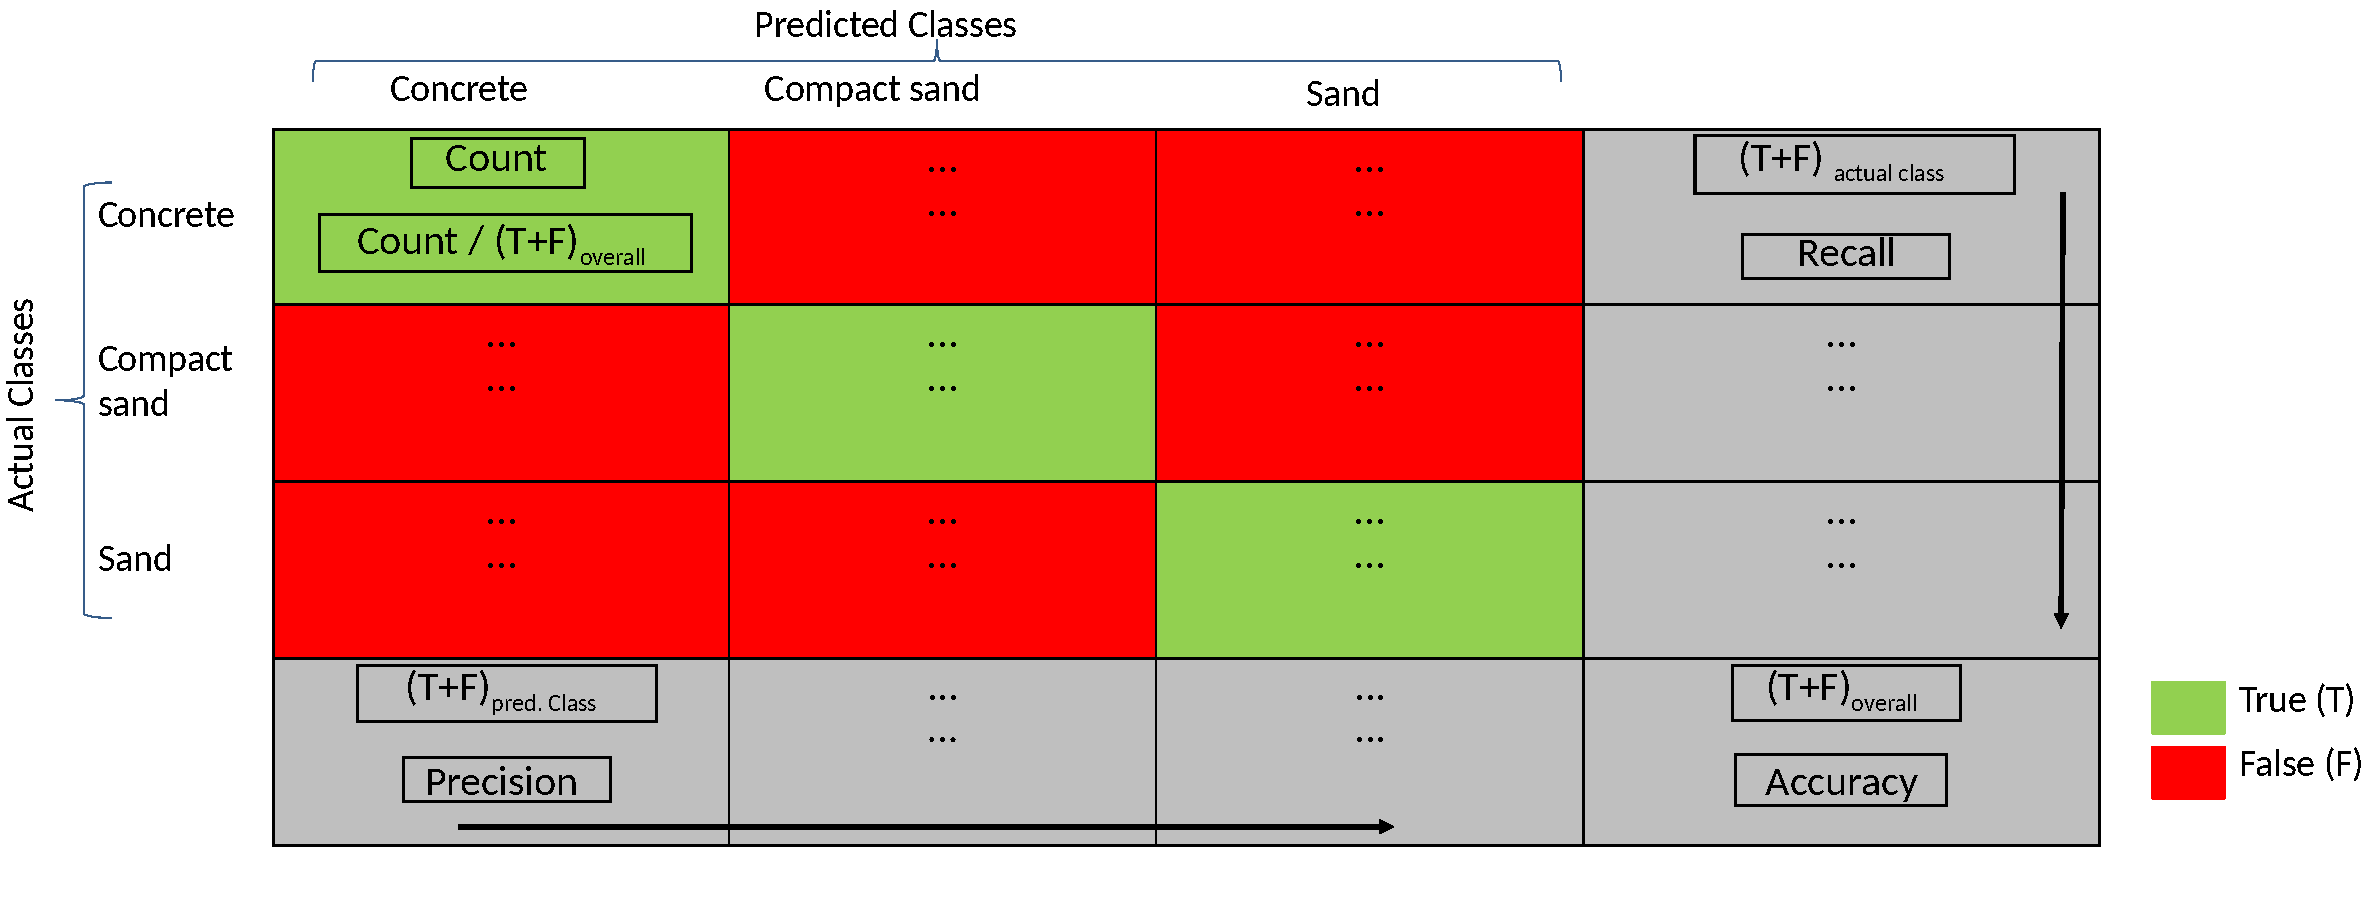
\includegraphics[width=\textwidth]{../figures/CM_Description.pdf}
\caption{\label{fig:CMdescrpit}Description of the used three class confusion matrix to visualize the three performance measures precision, recall and accuracy.\cite{kuhr2021}}
\end{figure}
\begin{itemize}
\item Accuracy $\frac{T\textsubscript{overall}}{(T+F)\textsubscript{overall}}$: Out of all samples tested, how many times does the classifier classify the correct class
\item Recall $\frac{T\textsubscript{class}}{(T+F)\textsubscript{actual class}}$: Out of all samples that belong to an actual class does the classifier classify the correct class 
\item Precision $\frac{T\textsubscript{class}}{(T+F)\textsubscript{predicted class}}$: Out of all classifications that the classifier assigns to one class does the classifier classify correctly
\end{itemize}

\subsubsection{Feature Selection}
For computational reasons and simplicity, it is desired to reduce the model's dimensionality by selecting the most critical features for the  classification task. 
Within the selection process, a large set of statistical moments of the features is considered. The features represent direct sensor parameter as well as physical parameter such as the mechanical and electrical power, three friction coefficients and the wheel speed deviation of each wheel in relation to the others. The thereby used proprioceptive sensor parameter are listed in Table~\ref{fig:features1}.
\begin{table}[htb!]
   \centering
    \caption{Acquired physical proprioceptive data from datastreams: MCS Logger (MCS), Joint Deployment Logger (JDL), Sensors Deployment Logger (SDL). The forces and torques are within the Body Coordinate System (BCS).\cite{Dimastrogiovanni2020}\label{fig:features1}}
    \begin{tabularx}{\columnwidth}{XXX}
    \textbf{Symbol}& \textbf{Feature} & \textbf{Datastream}  \\
    \hline
      $F\textsubscript{x}$ & Longitudinal Force	 &  MCS\\
      $F\textsubscript{z}$& Vertical Force	 &MCS \\ 
      $T\textsubscript{y}$& Drive Torque around y-axis	   &MCS\\ 
      $I $& Motor Current	  & JDL\\ 
      $V$ & Voltage 	   &JDL\\ 
      $d\textsubscript{pwm}$&  Dutycycle	   &JDL\\ 
      $w$& Angular Wheel Velocity 	 &JDL \\
      $a\textsubscript{x}$& Acceleration X	  &SDL\\ 
      $a\textsubscript{z}$&  Acceleration Z	   &SDL\\ 
    \end{tabularx}	
\end{table}
 In the following the formulas to calculate the physical parameter are presented:
\begin{itemize}
\item Mechanical Power: $ P\textsubscript{m} = T\textsubscript{y} * w $
\item Electrical Power: $ P\textsubscript{e} = V* I * d\textsubscript{pwm}$
\item Friction Coefficient 1: $\mu \textsubscript{1} = \frac{F\textsubscript{x}}{F\textsubscript{z}} $
\item Friction Coefficient 2: $\mu \textsubscript{2} = \frac{T\textsubscript{y}}{R * F\textsubscript{z}}$ 
\item Friction Coefficient 3: $\mu \textsubscript{3} = \frac{I}{R * F\textsubscript{z}}$
\item Speed Deviation:	 $\Delta w = |w-\overline{w}| $
\end{itemize}
$R$ represents SherpaTT's wheel radius which is $0.2085m$.
In this case, the statistical moments mean, variance, skewness and kurtosis are calculated. 
To reduce the dimensionality of inputs to the classifier, the most critical features for terrain classification are identified by using the WB index and the Pearson Coefficient as detailed in \cite{Dimastrogiovanni2020}. 
The list of selected features as well as which statistical moment is used is shown in Table~\ref{fig:optiF}.

\begin{table}[htb!]
   \centering
    \caption{Optimal feature set for the classification of terrain types by SherpaTT. The set includes the statistical calculation of mean (M) and standard deviation (SD) per terrain patch.\label{fig:optiF}}
    \begin{tabularx}{\columnwidth}{XXX}
    \textbf{Statistical} & \textbf{Feature}  & \textbf{Symbol} \\
    \hline
     M,SD	&  Longitudinal Force	 & F\textsubscript{x} \\ 
     M,SD	&  Drive Torque	around y-axis  & T\textsubscript{y} \\ 
     M,SD	&  Drive Current	 & I \\  
     M,SD	&  Acceleration X	 &  a\textsubscript{x}\\ 
     M,SD	&  Acceleration Z	 & a\textsubscript{z} \\ 
     M,SD	&  Mechanical Power	 & P\textsubscript{m} \\ 
     M,SD	&  Electrical Power	 & P\textsubscript{e} \\ 
     M,SD	&  Friction Coefficient 1	 & \textmu \textsubscript{1} \\ 
     M,SD	&  Friction Coefficient 2 & \textmu \textsubscript{2}\\ 
     M,SD	&  Friction Coefficient 3	 & \textmu \textsubscript{3}\\ 
     M	    &  Angular Wheel Velocity	     &  w      \\ 
     SD    	&  Speed Deviation	 & $\Delta$w\\ 
    \end{tabularx}	
\end{table}

\subsubsection{Linear Discriminant Analysis}
%copy paste from thesis
Besides speeding up the training and reducing the required amount of data during runtime, the reduction of feature dimensionality can help for data visualization. For this purpose, Linear Discriminant Analysis (LDA) reduces the number of dimensions down to three or two. This makes it possible to plot a high-dimensional data set on a graph and through this visually gain information about patterns. 

To achieve this, LDA identifies the axis that accounts for the largest amount of variance of different class's data. It thereby represents a similar method as the Principle Component Analysis (PCA) with the difference that LDA recognizes the class labels when identifying the variance. As a next step, LDA identifies the axis that lays orthogonal to the first one. Therefore, the second axis accounts for the largest amount of remaining variance. The maximum number of orthogonals, linear discriminants, depends on the number of dimensions within the data set.\cite{kuhr2021}



\section{Implementation}
\todo[inline]{RD: TODO for @RD: Add the diagrams and explanations of the software implementation, in particular showing how the data is taken on runtime from the streams fed to the classifier and delivered by the task port}

In this particular case, the classification takes place at a frequency of 100 $Hz$ which is also the highest input frequency (joint values), streams which have lower frequency, provide the same data to several input matrices. At a traverse speed of 0.1 $m/s$, one classification result per traversed 10 $cm$ is retrieved. 

Furthermore the classification results need to be available at a fast enough pace to allow other onboard components take advantage of the results (e.g. to improve navigation) and to ensure that the classification results correspond to the currently traversed surface. 
Likewise, the loss of data samples due to full queues on the input of the processing components must be avoided. 

The diagram in Figure~\ref{fig:overview} presents the implementation approach of the terrain classifier in Rock.

\begin{figure}[h]
\centering
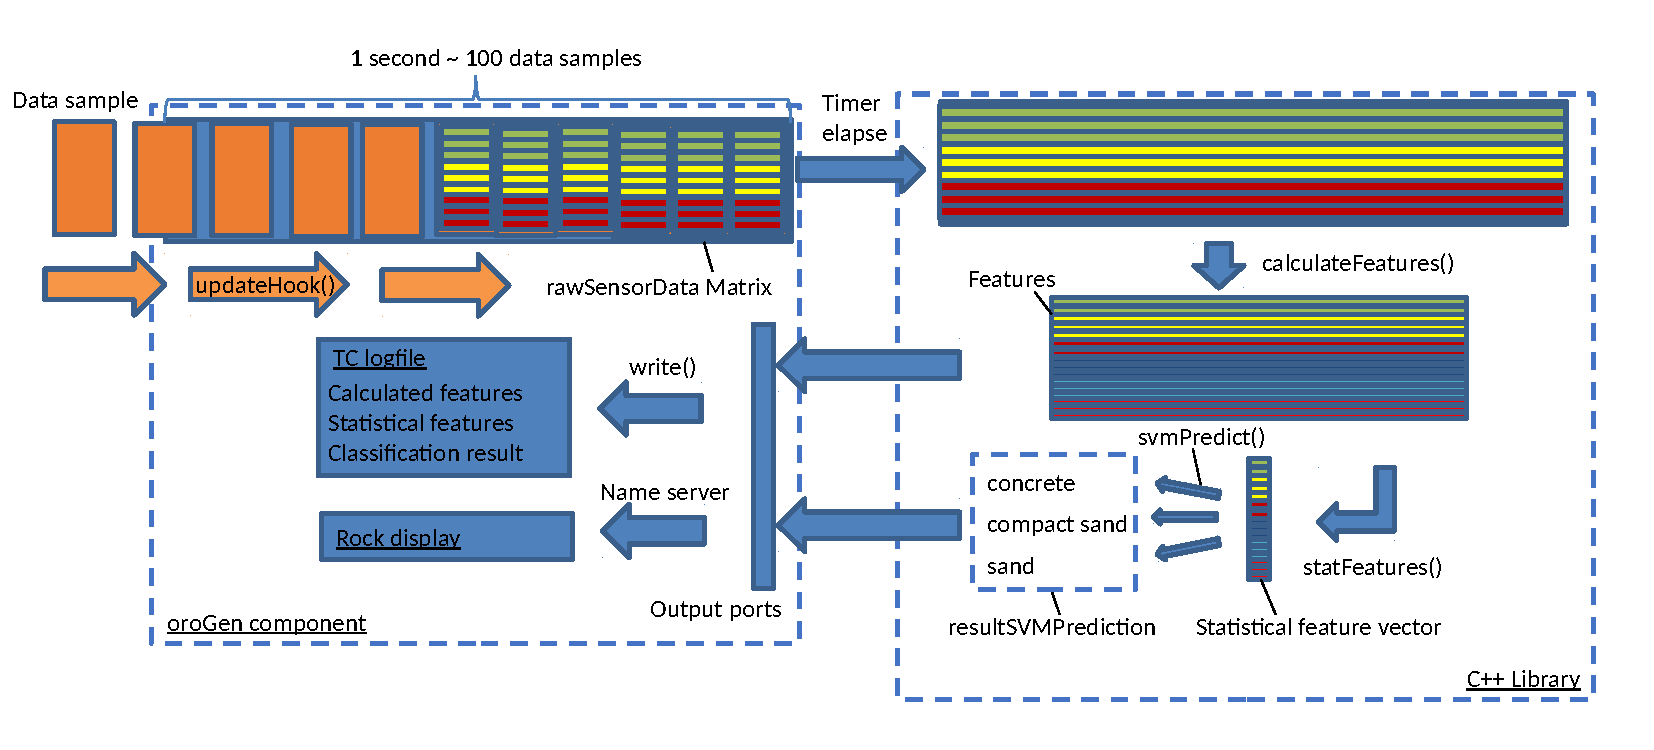
\includegraphics[width=\textwidth]{../figures/OverviewTC2.pdf}
\caption{\label{fig:overview}Overview of the terrain classifier library and Rock integration.}
\end{figure}

\subsection{Training Data}
\todo[inline]{RD: TODO for @LK: Explain the datasets that were collected for the training and how division between training and test data was done}

An essential aspect to the classification performance is a consistent and large data collection available for training. The data collection that is available for the implementation presented within this work
consists of data sets that were acquired from testruns on the three examined terrain types. Figure~\ref{fig:TestLocs} shows images of the traversed terrain during the test campaigns.

\begin{figure}[!htb]
    \begin{subfigure}[t]{0.33\textwidth}
        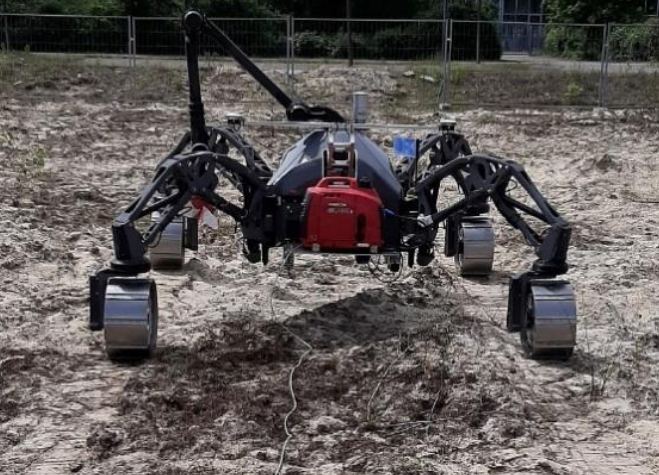
\includegraphics[width=\textwidth]{../figures/unprepsand.png}
        \caption{Loose Sand}
    \end{subfigure}
    \begin{subfigure}[t]{0.33\textwidth}
        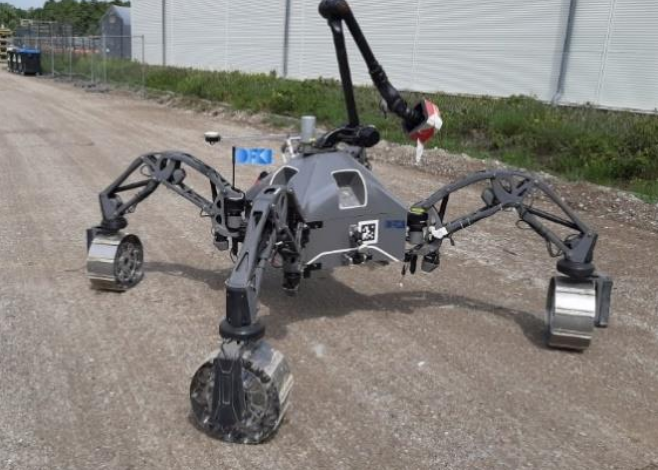
\includegraphics[width=\textwidth]{../figures/compact.png}
        \caption{Compact Sand}
    \end{subfigure}
    \begin{subfigure}[t]{0.33\textwidth}
        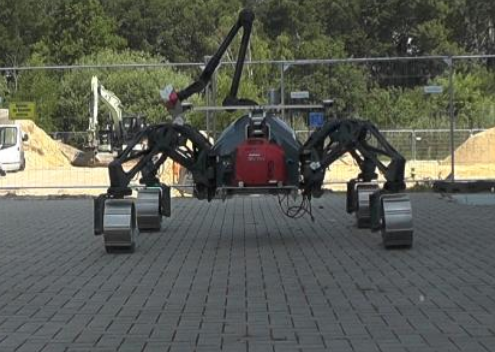
\includegraphics[width=\textwidth]{../figures/concrete.png}
        \caption{Concrete}
    \end{subfigure}
 \caption{The test locations where the data sets were acquired.}
 \label{fig:TestLocs}
\end{figure}

One testrun corresponds to the forward or backward driving for a defined distance. The test conditions were the same during all testruns. Such test conditions are:
\begin{itemize}
\item Fixed wheel configuration
\item Surface of no inclination
\item Traverse speed 0.1 $m/s$
\item Straight traverses/ no turns
\item Power generator is on
\item Traverse 10 $m$ per testrun
\end{itemize}

In terms of quantity, the data collection consists of 2200 training samples for each of the 76 features. Regarding data balance, the data gathered from the terrain type sand represent 28\% of the data and the concrete and compact sand represent 36\% each. 
When generating a SVM model the available data collection one of the data sets of each terrain traverse is used for testing and the others are used for training. This gives a relation of about 25/75.






\section{Evaluation}
\subsection{Offline Classification Performance}
\todo[inline]{RD: TODO for @LK: Provide the results that were collected when testing offline}
%The SVM model training software is implemented to enable the use of a variable constellation of logged datasets. Moreover, it can be used to compare both the offline and online classification performance. 

The offline evaluation of the SVM classifier reached an accuracy of 93.97\% as shown in the confusion matrix in Figure~\ref{fig:confusionmatrix}. A small portion of the testrun data is collected even when SherpaTT is not moving. The datapoints for which the wheel speed is zero are sliced out. Based on the sliced data  the classification accuracy could be increased by 2\%.

\begin{figure}[h]
\centering
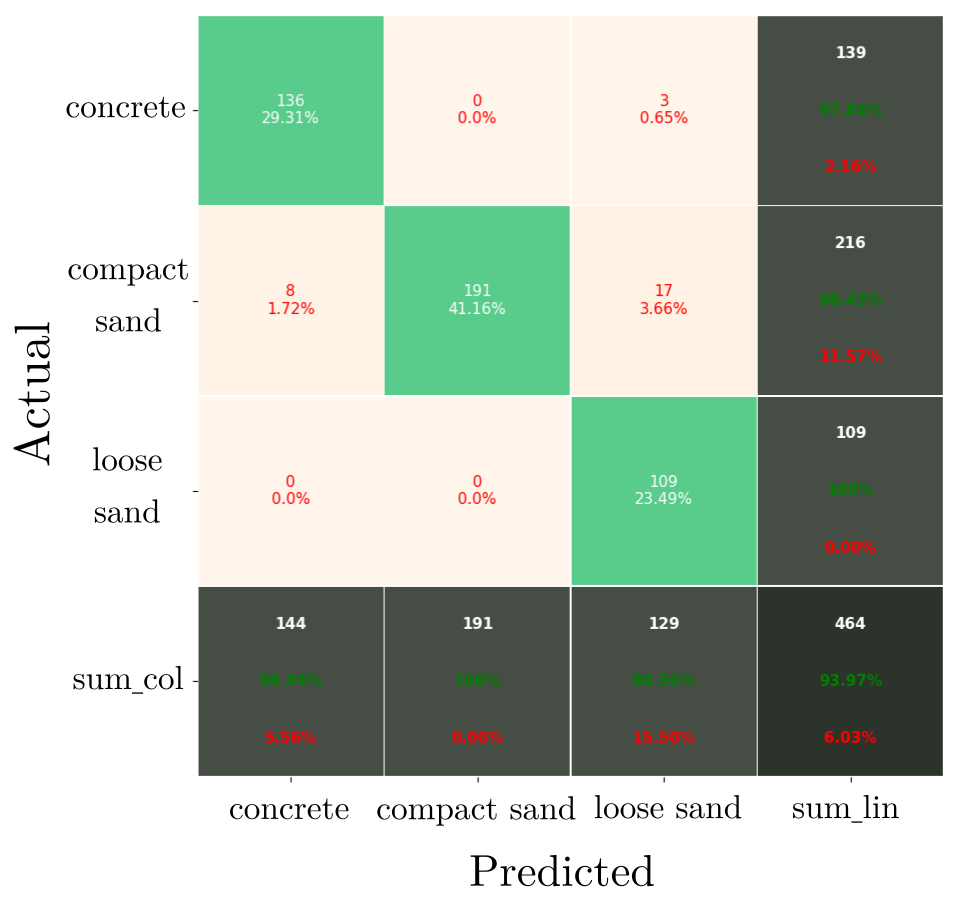
\includegraphics[width=0.5\textwidth]{../figures/confusionmatrix_Train.png}
\caption{\label{fig:confusionmatrix} Shows the performance of the SVM model. Except the recall for \emph{compact sand} and the precision for \emph{sand} all performances are above 90\%, with an overall accuracy of 93.97\%}
\end{figure}

To visualize the achieved data separation the components of a LDA are plotted . Figure~\ref{fig:lda} shows the resulting plot highlighting the decision boundary of the used linear SVM kernel as well. It is shown that the data of the terrain types can be separated for most of the samples.
\begin{figure}[!htb]
 \centering
 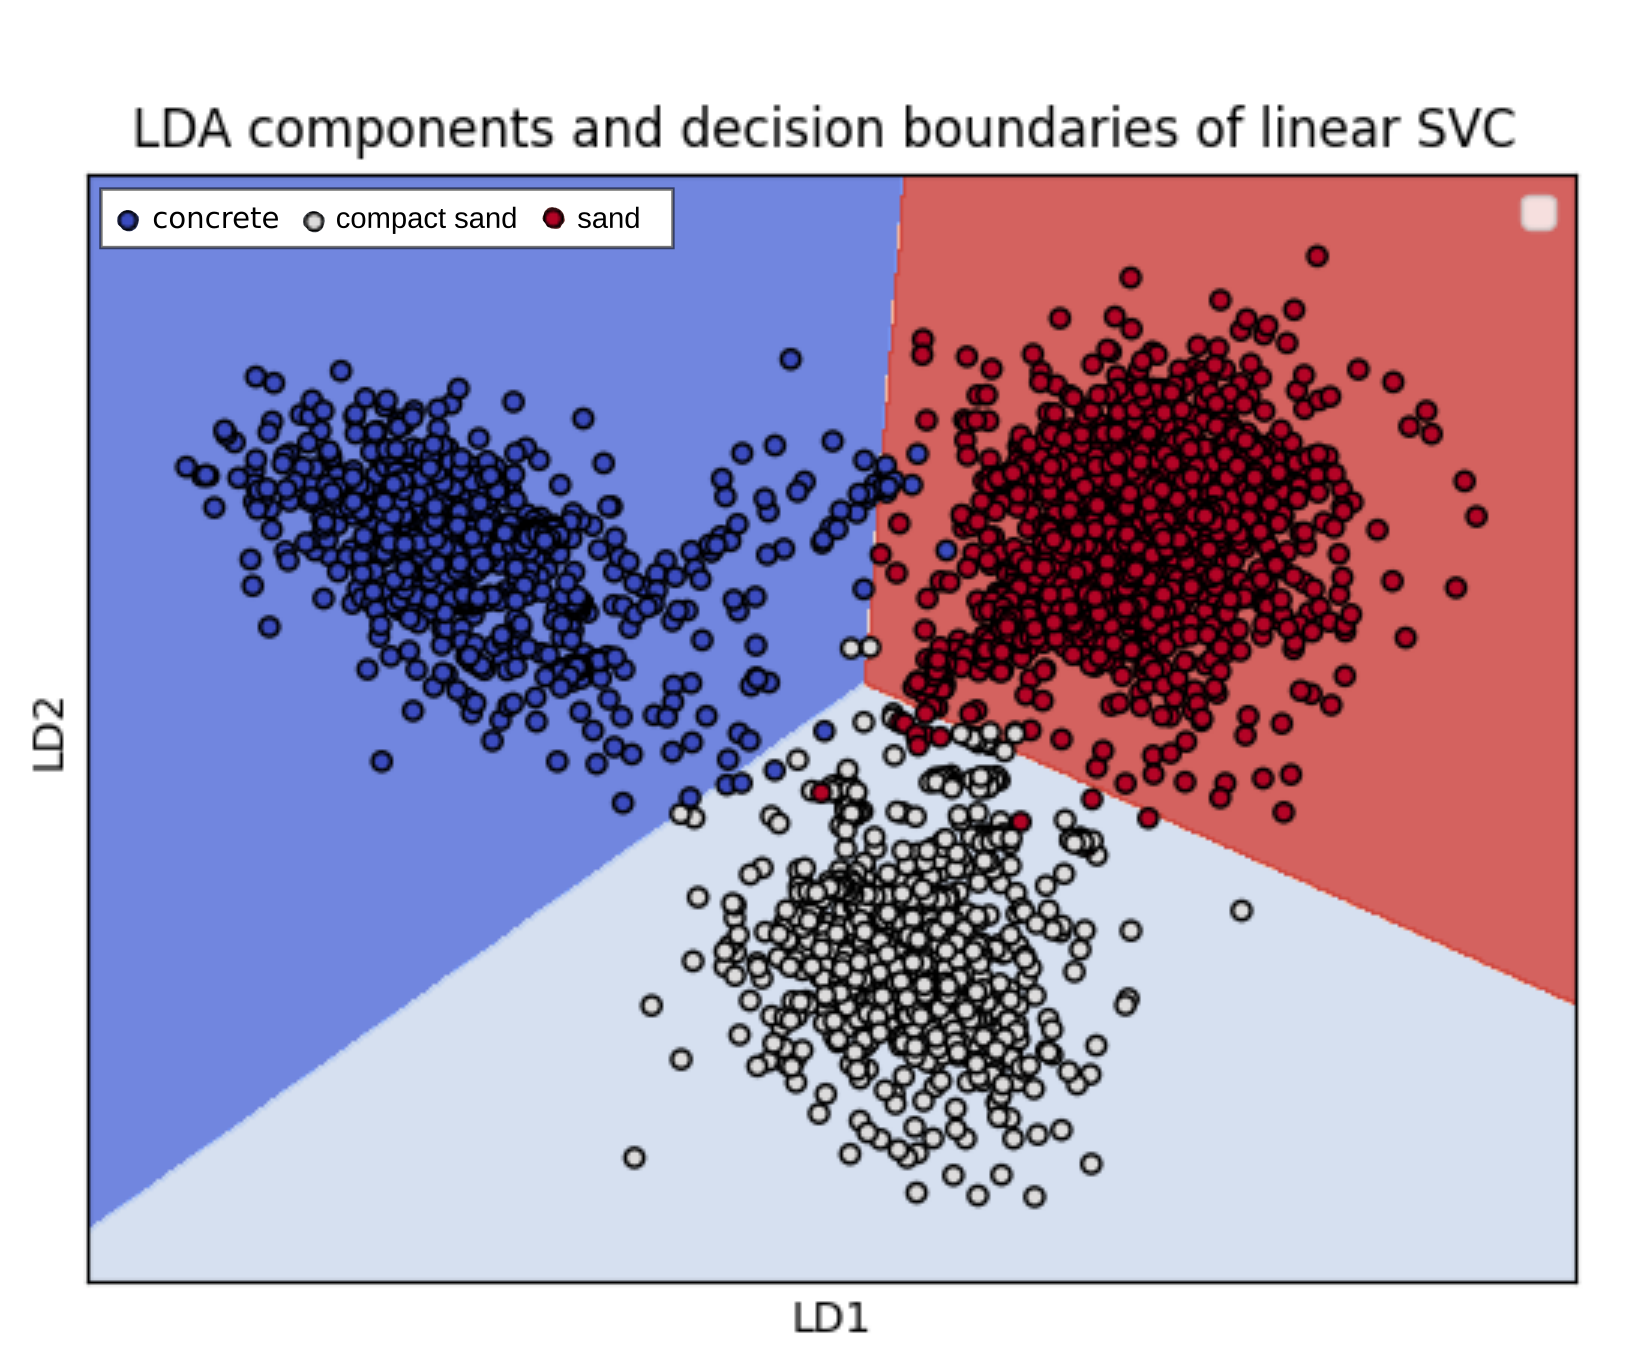
\includegraphics[width=0.9\textwidth]{../figures/boundary_LDA_prevTesting_all_sand_concrete_compactsand.png}
 \caption{Shows a plot with the two Linear Discriminant (components) on the axes. The dimensions of the original feature set is reduced to two. The data samples of all available data sets are displayed. Also the decision boundary generated by a Support Vector Kernel (SVC) is displayed. The areas of different terrain types are highlighted by the corresponding colors. }
 \label{fig:lda}
\end{figure}



% Evaluation




%A complete analysis of performance was not possible, because the traversed terrain during the field tests did not closly match the previously trained terrain classes. Nevertheless, the software shows good classification results, since the type of surface -\emph{wet compact sand}- was close to the two classes mostly identified -\emph{concrete} and \emph{compact sand}.

\subsection{Online tests}
\todo[inline]{RD: TODO for @LK and @RD: Explain the tests that were performed outdoors}

Two main tests were performed to validate the onboard calculation of features and classification performance.
The tests consisted of traverses where the component was executing along with the rest of the control and perception sofware components. 
The first of the test was perfomed indoors at the DFKI Robotics Innovation Center premises, depicted in Figure~\ref{fig:sh-tests}.
During the test the classifier run at the pursued frequency of 100Hz.
Here the classification performance is not considered representative since the power generator was not active and the hardest surface was not as hard as concrete. 

\begin{figure}[!htb]
    \centering
    \begin{subfigure}[t]{0.45\textwidth}
        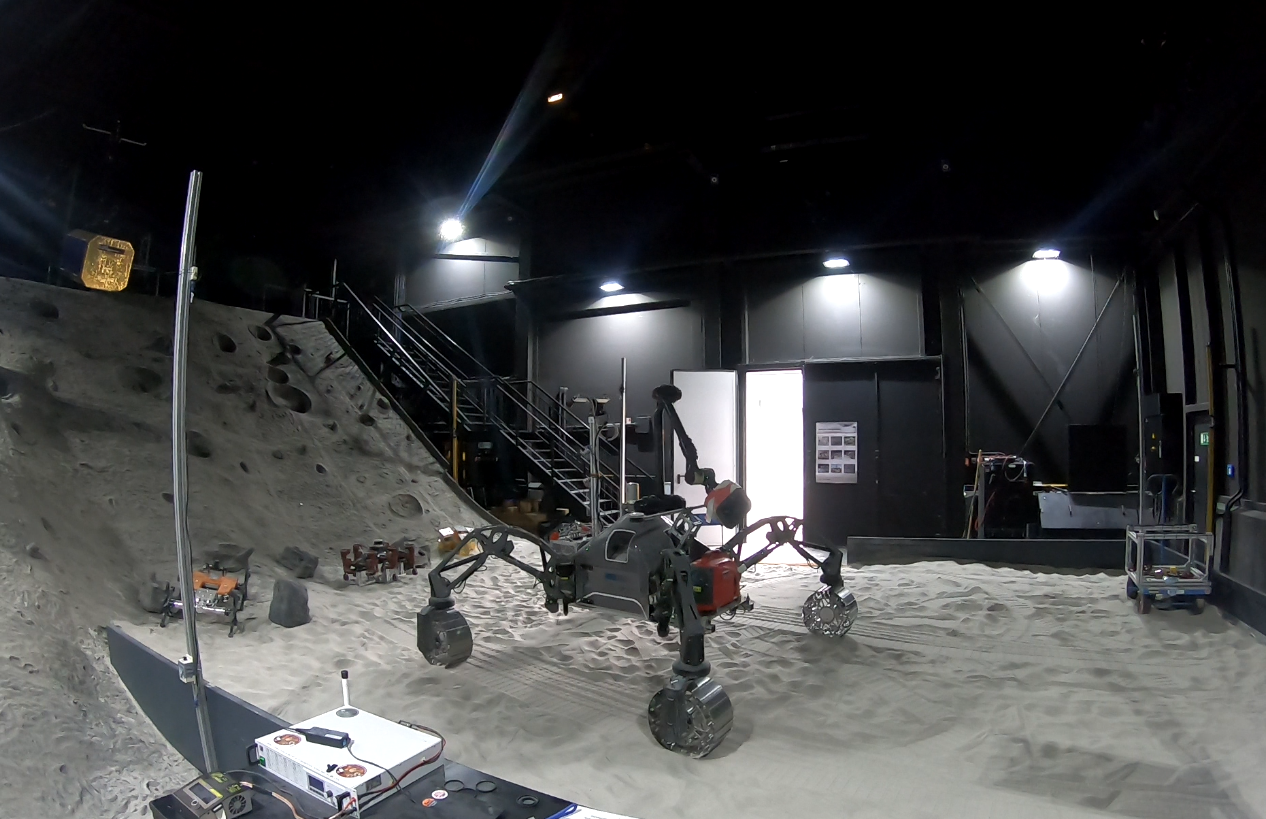
\includegraphics[width=\textwidth]{../figures/spacehall.png}
        \caption{Loose Sand Test}
    \end{subfigure}
    \begin{subfigure}[t]{0.45\textwidth}
        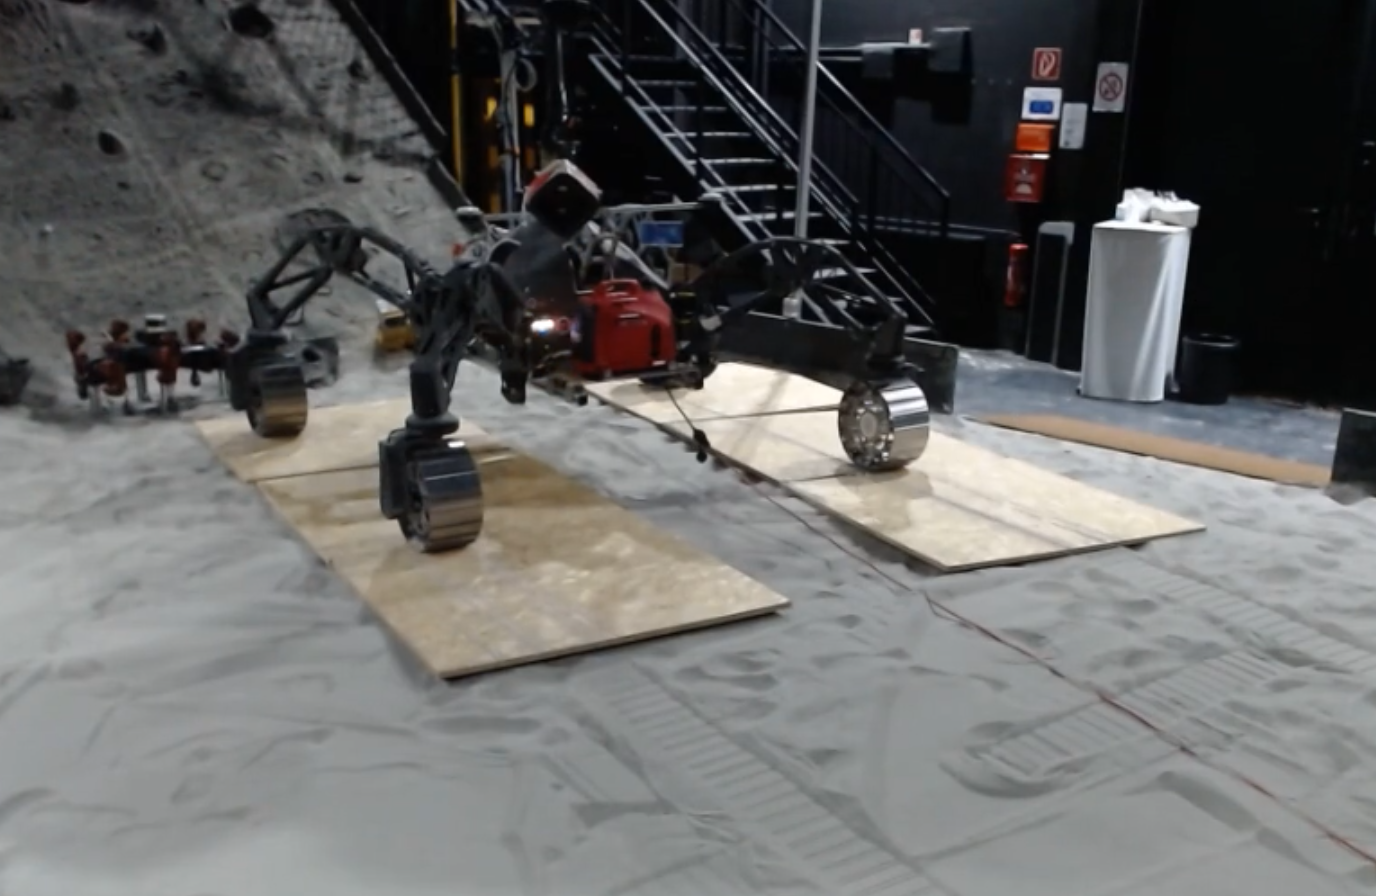
\includegraphics[width=\textwidth]{../figures/spacehallconcrete.png}
        \caption{Concrete Test}
    \end{subfigure}
    \caption{First onboard tests to validate the requirements on execution frequency}
    \label{fig:sh-tests}
\end{figure}

The second test was during the final field tests of the ADE project \cite{ocon2021} in a sand mine in the north of Germany.
These tests allowed to provide comparable surface traverse conditions as ones within the training data, since the power generator was activated.
To check that the feaute calculations were correct, several traverses of SherpaTT were logged and checked for consistency. 
The classification accuracy reached 87\% and a well balanced recall and precision values of the classes was achieved. 
The underperformance in the field test conditions was due to the nature of the surface, which did not physically match any of the previously examined types. 
The field test surface consisted of wet compact soil, which furthermore was getting attached to the wheels Figure~\ref{fig:finaltest}.
Nevertheless, the classification was mostly as compact sand or concrete, the closest classes that the classifier was trained with.
Moreover, it was demonstrated that the terrain classifier can be executed onboard of SherpaTT and that it is able to compute the correct features as well as classify different terrain types successfully, whilst the rover is traversing.


\begin{figure}[!htb]
 \centering
 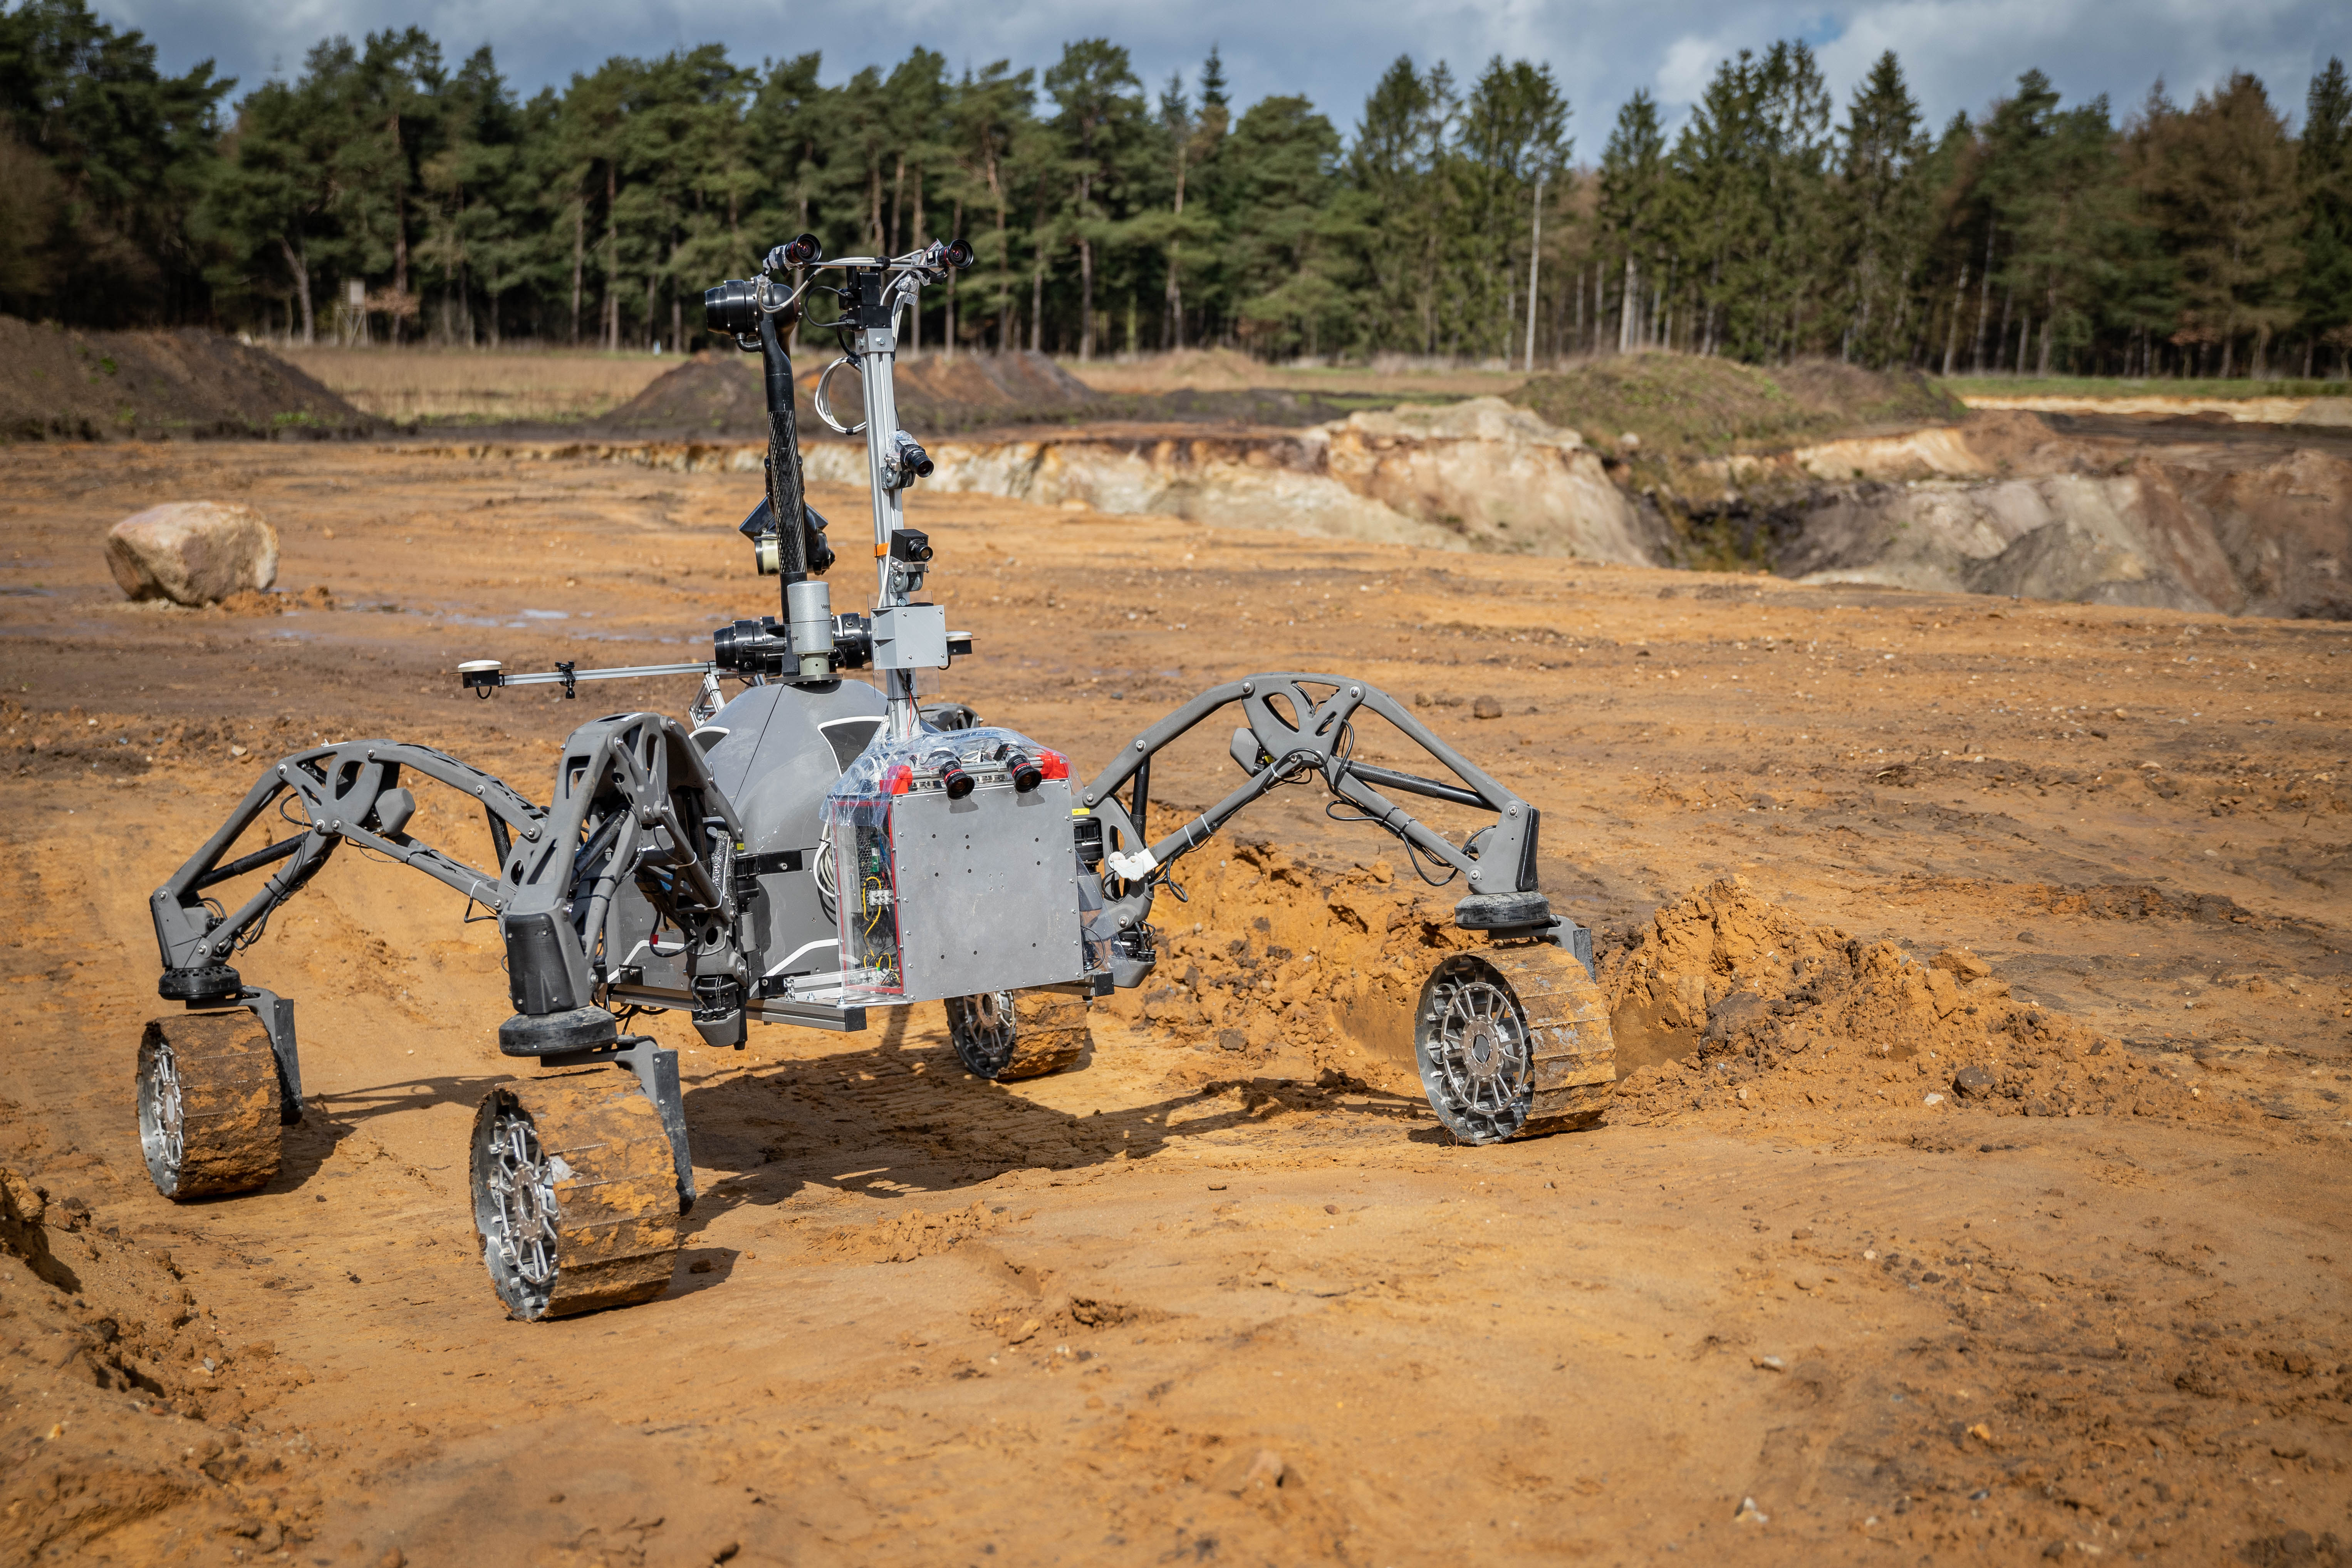
\includegraphics[width=0.9\textwidth]{../figures/sandmine.png}
 \caption{The analog site where the classifier was tested had surfaces with features different to those seen in the training sets}
 \label{fig:finaltest}
\end{figure}


\subsubsection{Computational Performance}
\todo[inline]{RD: TODO for @LK Some clarifications and numbers on the performance checks done through software: wall\_time and cpu\_time}


%The C++ calculations and terrain classifications were executed in sufficient time in parallel to the rest of SherpaTT's Motion Control System, on a single thread, using a i7 processor with a CPU clock speed of 4.6 GHz.
The implementation foresees to repeatedly measure the execution time of the code. In the case of this implementation the computation is executed on a single thread. Consequentially, the execution time can be identified measuring the averaged wall time of the code execution. Table 4.3 shows the results of these measurements. 
\begin{table}[htb!]
   \centering
    \caption{Shows the results of wall time measurements of the methods of the C++ library.}\label{fig:compmeasurments}
    \begin{tabularx}{\columnwidth}{X|XXX}
    \textbf{Method:} & \multicolumn{3}{X}{Wall Time [$ms$]} \\
    &min.&max.&avg.\\
    \hline
    \hline
\textbf{calculateFeatures():} & 9&  17.1& 13.2 \\
\textbf{calculateStat():}     & 6.3 & 13 & 7.1 \\
\textbf{svmPredict():}        &  0. &  0.001 & 0.0007  \\
\hline
\textbf{overall:}             & 15.3 & 30.1 &20.3  \\
    \end{tabularx}	
\end{table}
Since the execution time depends on the system on which the code executed, the computational system specification need to resemble those of SherpaTT. Moreover, the resulting execution time depends
on the threading of the operating system which is in this case the Linux distribution Ubuntu. The specification is a i7 processor with a CPU clock speed of 4.6 GHz. 

As the averaged execution time of the C++ library is 20.3 $ms$ this could potentially lead to the delay of two \texttt{updateHook()} triggerings which are done every 10 $ms$, and hence the drop of one data sample per second. The drop of one data sample of the one hundred data samples that are strapped every second is assumed to be acceptable.

\section{Conclusions}
\todo[inline]{RD: TODO for @RD Wrap up and outlook}


\FloatBarrier

\bibliographystyle{alpha}
\bibliography{sherpatt_terrain_classifier.bib}

\end{document}
